\chapter{Модель активации теплоносителя первого контура}

\section{Миграция радионуклидов на \ac{aes}}
\label{sec_nuclides_migration}

Как и любое масштабное производство, \ac{aes} выбрасывает в атмосферу и окружающую среду вредные вещества, среди 
которых есть и радиоактивные. При нормальных условиях эксплуатации эти выбросы незначительны, так как современные 
атомные электростанции содержат множество систем очистки сбросов от радионуклидов, однако при нарушении работы 
какой-либо из систем \ac{aes} становится серьезным источником выбросов радионуклидов в атмосферу. 

Хотя принцип работы различных типов ядерных реакторов одинаков, их технологические схемы и устройства различны. В 
данном разделе рассмотрим образование радионуклидов с дальнейшим переходом в теплоноситель первого контура на примере 
реактора типа \ac{vver}.

Основные пути распространения радиоактивных нуклидов на \ac{aes} представлены на рисунке \ref{fig_nuclides_spread}.

\begin{figure}[ht]
\centering
	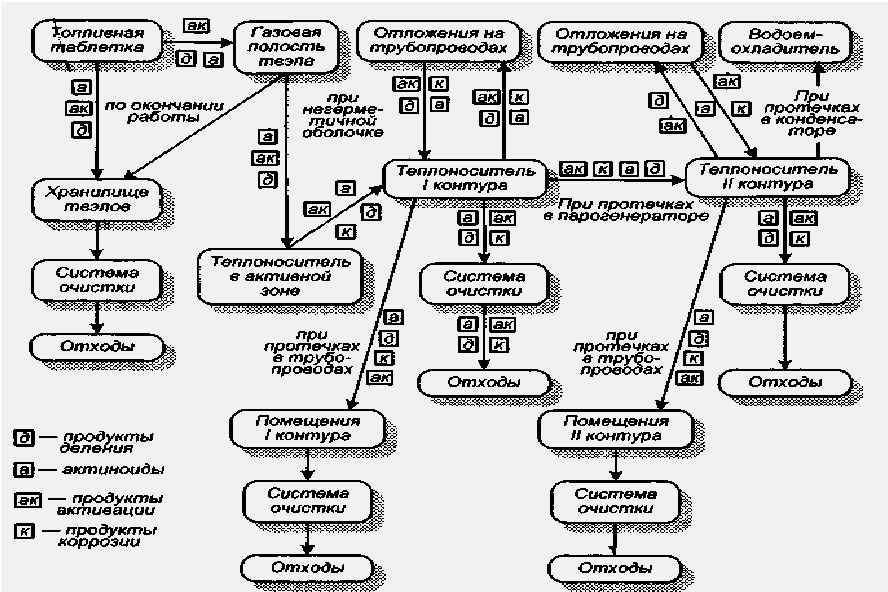
\includegraphics[width=16cm]{nuclides_spread}
	\captionsetup{justification=centering}
    \caption{Основные пути распространения радионуклидов на \ac{aes}.}
    \label{fig_nuclides_spread}
\end{figure}

Топливную таблетку в \ac{tvel}ах рассматривают как первый барьер распространения радиоактивных нуклидов в пределах 
активной зоны ядерного реактора. В результате реакции деления и захвата нейтронов в топливной таблетке накапливаются 
радионуклиды, изменяя состав, физико-химические и механические свойства топливной композиции. При температуре ниже 
1000 \degree C диоксид урана, который наиболее часто используется в качестве топлива в реакторах типа \ac{vver}, 
удерживает все радионуклиды, образующиеся в процессе работы реактора. При росте температуры ситуация существенно 
меняется, так как продукты захвата и деления становятся более подвижными \cite{leskin_vver}.

Между топливной таблеткой и оболочкой \ac{tvel}а присутствует небольшой зазор и газовая полость, предназначенные для 
накопления продуктов деления и активации, которым удалось покинуть пределы топливной таблетки.

Вторым барьером распространения радионуклидов является оболочка \ac{tvel}ов. В случае герметичной оболочки \ac{tvel}ов 
выход радионуклидов за пределы оболочки достаточно мал. В реальности, из за высоких тепловых и радиационных нагрузок и 
процессов коррозионно-усталостного типа оболочки теряют свою герметичность. Согласно \cite{kolpakov_tvel}, при 
эксплуатации ядерного реактора пределом безопасной эксплуатации по количеству и величине дефектов составляет 1 \% 
\ac{tvel}ов с дефектами типа газовой неплотности.

В случае разгерметизации топливной оболочки радионуклиды диффундируют через микротрещины в теплоноситель, находящийся 
в активной зоне реактора, который в дальнейшем переходит в первый контур реакторной установки. Более того, 
дополнительным источником радиоактивности в теплоносителе первого контура является его активация нейтронами. 

При эксплуатации \ac{aes} в нормальном режиме работы обеспечивается локализация радиоактивных продуктов деления, 
продуктов активации в реакторной установке и основных системах очистки от радиоактивных нуклидов. Парогенератор и 
трубопроводы первого и второго контуров не позволяют значительной части радионуклидов покинуть основные барьеры. Однако
при наличии микротрещин или протечек в парогенераторе радиоактивность первого контура может перейти в теплоноситель 
второго контура реакторной установки. В то же время, при протечках в трубопроводах первого или второго контура 
радионуклиды попадают в технические помещения, а далее загрязненный воздух через вентиляционные системы выбрасывается 
в атмосферу. Газообразные выбросы с \ac{aes} перед попаданием в атмосферу проходят сложную систему очистки, которая в 
свою очередь необходима для снижения активности выбросов, а далее попадают в окружающую среду через высокую трубу.

Помимо газообразных радиоактивных отходов при работе реактора выделяются жидкие и твердые отходы (рисунок 
\ref{fig_nuclides_spread2}). Твердыми радиоактивными отходами являются конструкционные материалы из активной зоны и 
первого контура, фильтры очистки установок, загрязненные инструменты, приборы и т.д. Твердые радиоактивные отходы после 
эксплуатации отправляются на захоронение. Жидкие радиоактивные отходы также образуются в результате эксплуатации 
\ac{aes}, в дальнейшем их очищают, разбавляют, фильтруют или концентрируют и хранят в специальных емкостях в жидком 
виде, однако при протечках в парогенераторе и конденсаторе радиоактивные отходы, мигрировавшие во второй контур 
реакторной установки, могут попасть в водоем-охладитель \cite{bekman_nuclear}. 

\begin{figure}[ht]
	\centering
	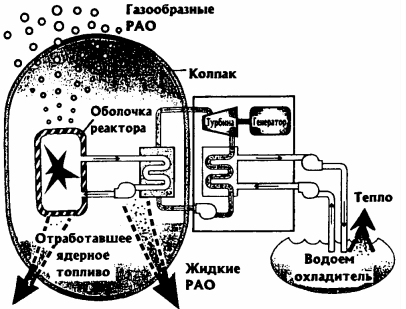
\includegraphics[width=10cm]{nuclides_spread2}
	\captionsetup{justification=centering}
    \caption{Схема образования газообразных, жидких и твердых отходов от \ac{aes} \cite{bekman_nuclear}.}
    \label{fig_nuclides_spread2}
\end{figure}

\section{Образование газообразных радионуклидов \ac{aes}}
\label{sec_gas_nuclides}

Рассмотрим наиболее важные радионуклиды, которые образуются в процессе работы реакторной установки и потенциально 
могут попасть в атмосферу путем газообразных выбросов \ac{aes}. 

Важную роль в формировании радиационной обстановке в районе выбросов \ac{aes} являются инертные радиоактивные газы. 
\ac{irg} попадают в теплоноситель при разгерметизации оболочек \ac{tvel}ов путем диффузии. Более десятка нуклидов 
инертных радиоактивных газов (криптона и ксенона) образуется в процессе деления нейтронами ядерного топлива 
\cite{bekman_nuclear}, а так же при распаде других продуктов реакции деления. Часть радионуклидов имеют либо малый 
период полураспадам (меньше минуты), либо вносят ничтожно малый вклад в суммарную активность, из-за чего их можно не 
учитывать в расчетах. Основные радионуклиды и их периоды полураспада \ac{irg}, образующиеся в процессе работы реактора, 
представлены в таблице \ref{table_irg}. В реакторах типа \ac{vver} инертные радиоактивные газы могут поступать в 
атмосферу путем утечки воды из первого контура реакторной установки или при утечке воды из второго контура реакторной 
установки при протечках в парогенераторе. 

\begin{table}[ht]
	\setlength{\extrarowheight}{1mm}
	\caption{Основные радионуклиды \ac{irg}, образующиеся в процессе работы реактора \cite{gusev_bio}.}
	\label{table_irg}
	\centering
    \begin{tabular}{|M{0.4\textwidth}|M{0.4\textwidth}|}
    \hline Нуклид & $\text{T}_{1/2}$ \\
    \hline $^{133}\text{Xe}$ & 5,21 суток \\
    \hline $^{135}\text{Xe}$ & 9,14 часов \\
    \hline $^{137}\text{Xe}$ & 3,9 минут \\
    \hline $^{138}\text{Xe}$ & 17,5 минут \\

    \hline $^{85}\text{Kr}$ & 10,76 лет \\
    \hline $^{87}\text{Kr}$ & 76 минут \\
    \hline $^{88}\text{Kr}$ & 2,8 часов \\   
    \hline 
    \end{tabular}
\end{table}

Стоит отметить, что радионуклиды, период полураспада которых намного меньшим кампания реактора ($^{137}\text{Xe}, 
^{87}\text{Kr}$) в ходе работы реактора быстро достигают состояния насыщения и их количество не меняется со временем. В 
то же время долгоживущие радионуклиды, период полураспада которых близок или превышает кампанию реактора 
($^{85}\text{Kr}$) накапливаются в топливе практически линейно со временем \cite{naumov_security}.

Не менее важными газообразными радионуклидами, попадающими в атмосферу, являются изотопы иода. Изотопы иода в ядерном 
реакторе образуются в результате реакции деления, а так же при распаде продуктов деления топлива. Пути попадания 
радиоактивных изотопов иода в атмосферу аналогичны инертным радиоактивным газам. Основные радионуклиды иода, 
образующиеся в процессе работы реактора, представлены в таблице \ref{table_iod}.

\begin{table}[ht]
	\setlength{\extrarowheight}{1mm}
	\caption{Основные радионуклиды иода, образующиеся в процессе работы реактора \cite{gusev_bio}.}
	\label{table_iod}
	\centering
    \begin{tabular}{|M{0.4\textwidth}|M{0.4\textwidth}|}
    \hline Нуклид & $\text{T}_{1/2}$ \\
    \hline $^{131}\text{I}$ & 8,05 суток \\
    \hline $^{132}\text{I}$ & 2,26 часов \\
    \hline $^{133}\text{I}$ & 20,3 часов \\
    \hline $^{134}\text{I}$ & 52 минут \\
    \hline $^{135}\text{I}$ & 6,68 часов \\   
    \hline 
    \end{tabular}
\end{table}

Из-за небольшого периода полураспада, в реакторе для вышеперечисленных радионуклидов достаточно быстро устанавливается 
равновесное состояние. Исключение составляет изотоп $^{129}\text{I}$ ($\text{T}_{1/2} = 1.57 \times  10^7$ лет), однако 
согласно \cite{bekman_nuclear} долгожвущий иод не обнаруживают в атмосфере и окружающей среде вокруг \ac{aes} и его 
выбросы во много раз меньше выбросов других радионуклидов иода.

Некоторые продукты деления ядер топлива, продукты распада \ac{irg} и радионуклиды с наведенной активностью образуют 
аэрозоли, которые попадают во внешнюю среду с воздушными потоками. Наиболее важные радионуклиды, которые входят в 
состав аэрозольных выбросов с реактора типа \ac{vver}, представлены в таблице \ref{table_aero}. 

\begin{table}[ht]
    \setlength{\extrarowheight}{1mm}
    \caption{Основные радионуклиды, входящие в состав аэрозолей, образующиеся в процессе работы реактора 
        \cite{bekman_nuclear}.}
    \label{table_aero}
    \centering
    \begin{tabular}{|M{0.4\textwidth}|M{0.4\textwidth}|}
    \hline Нуклид & $\text{T}_{1/2}$ \\
    \hline $^{88}\text{Rb}$ & 18 минут \\
    \hline $^{134}\text{Cs}$ & 2,07 лет \\
    \hline $^{137}\text{Cs}$ & 30,17 лет \\
    \hline $^{138}\text{Cs}$ & 33 минуты \\
    \hline $^{60}\text{Co}$ & 5,27 лет \\   
    \hline 
    \end{tabular}
\end{table}

В процессе работы реактора образуются активационные газы - изотопы $^{16}\text{N}$ и $^{41}\text{Ar}$. Изотоп 
$^{16}\text{N}$ образуется в реакторе из $^{16}\text{O}$ в ходе реакции (n, p) (в реакторе \ac{vver} кислород 
содержится либо в оксидном топливе, либо в теплоносителе), а $^{41}\text{Ar}$ образуется при облучения нейтронами 
изотопа $^{40}\text{Ar}$, растворенного в теплоносителе вместе с воздухом, в ходе реакции (n, $\gamma$). Периоды 
полураспада основных активационных газов представлены в таблице \ref{table_active_gas}.

\begin{table}[ht]
    \setlength{\extrarowheight}{1mm}
    \caption{Основные активационные газы, образующиеся в процессе работы реактора 
        \cite{bekman_nuclear}.}
    \label{table_active_gas}
    \centering
    \begin{tabular}{|M{0.4\textwidth}|M{0.4\textwidth}|}
    \hline Нуклид & $\text{T}_{1/2}$ \\
    \hline $^{41}\text{Ar}$ & 1,83 часов \\
    \hline $^{16}\text{N}$ & 7,13 секунд \\
    \hline 
    \end{tabular}
\end{table}

Радиоактивный углерод $^{14}\text{C}$ образуется в реакторе по трём основным каналам: активация нейтронами естественных 
карбидных солей в теплоносителе первого контура, содержащих $^{13}\text{C}$, в ходе (n, $\gamma$) реакции; активация 
азота $^{14}\text{N}$, находящегося в виде примеси в топливе, в ходе (n, p) реакции; активация кислорода, содержащегося 
в оксидном топливе и в теплоносителе первого контура, в ходе (n, $\alpha$) реакции. Период полураспада изотопа 
$^{14}\text{C}$ составляет 5730 лет \cite{bekman_nuclear}.

Газообразный тритий образуется так же по трём основным каналам: при тройном делении ядер топлива (маловероятный процесс, 
из-за чего в расчетах можно принебречь им); в результате активации нейтронами ядер $^{6}\text{Li}$ и $^{10}\text{B}$, 
которые растворены в теплоносителе первого контура, в ходе реакций $^{6}\text{Li}$(n, $\alpha$)$^{3}\text{H}$ и 
$^{10}\text{B}$(n, $2\alpha$)$^{3}\text{H}$; в ходе активации дейтерия, содержащегося в теплоносителе в качестве 
примеси. Период полураспада трития составляет 12,32 лет \cite{bekman_nuclear}.

\section{Активация теплоносителя радионуклидами, выходящими из под оболочки \ac{tvel}ов}
\label{sec_tvel_nuclides}

Как было сказано в разделе \ref{sec_gas_nuclides}, в случае разгерметизации оболочек \ac{tvel}ов в теплоноситель 
первого контура могут попасть следующие радионуклиды, образующиеся в результате реакции деления ядер топлива: изотопы 
иода ($^{131}\text{I}$, $^{132}\text{I}$, $^{133}\text{I}$, $^{134}\text{I}$, $^{135}\text{I}$), изотопы, входящие в 
состав аэрозолей ($^{134}\text{Cs}$, $^{137}\text{Cs}$, $^{138}\text{Cs}$, $^{88}\text{Rb}$), инертные радиоактивные 
газы ($^{133}\text{Xe}$, $^{135}\text{Xe}$, $^{137}\text{Xe}$, $^{138}\text{Xe}$, $^{85}\text{Kr}$, $^{87}\text{Kr}$, 
$^{88}\text{Kr}$), а так же тритий ($^{3}\text{H}$).

Изменение концентрации i-ого нуклида, который образуется под оболочкой твэла в результате деления, определяется формулой 
\ref{eq_tvel_conc}.

\begin{equation}
    \label{eq_tvel_conc}
    \frac{\partial c_{i}}{\partial t} = -\lambda_{i}c_{i} + \gamma_{i}\Sigma_{f}\phi - S_{i}
\end{equation}

где:
\begin{description}
    \item $\text{c}_i$ --- концентрация i-го нуклида под оболочкой \ac{tvel}а;
    \item $\lambda_{i}$ ---  постоянная распада i-ого нуклида;
    \item $\gamma_{i}$ --- вероятность выхода i-ого нуклида при реакции деления;
    \item $\Sigma_{f}$ --- макроскопическое сечение деления ядер топлива;
    \item $\phi$ --- поток нейтронов;
    \item $\text{S}_{i}$ --- вероятность выхода i-ого нуклида из-под оболочки \ac{tvel}а.
\end{description}

В левой части уравнения \ref{eq_tvel_conc} - скорость изменения концентрации i-ого нуклида под оболочкой \ac{tvel}а, 
которая представлена в виде суммы трех слагаемых: скорости распада нуклида, скорости образования нуклида в результате 
деления ядер топлива и скорости увода нуклида через микротрещина разгерметизированных оболочек \ac{tvel}ов в 
теплоноситель первого контура.

Уравнение \ref{eq_coolant_balance} описывает баланс между концентрацией i-ого нуклида в теплоносителе первого контура 
без учета его очистки и выходом i-ого нуклида из-под оболочки \ac{tvel}ов:

\begin{equation}
    \label{eq_coolant_balance}
    S_{i}^{0} = \lambda_{i}\widetilde{c}_{i}^{0}\frac{V_{coolant}}{V_{core}}
\end{equation}

где:
\begin{description}
    \item $\widetilde{c}_{i}^{0}$ --- равновесная концентрация i-ого нуклида в теплоносителе первого контура;
    \item $S_{i}^{0}$ --- равновесный выход i-ого нуклида из-под оболочки \ac{tvel}ов, при котором в 
        теплоносителе первого контура будет установлена концентрация $\widetilde{c}_{i}^{0}$ i-ого нуклида;
    \item $V_{coolant}$ --- объем теплоносителя первого контура;
    \item $V_{core}$ --- объем активной зоны.
\end{description}

Выход радионуклидов через оболочку зависит от множества параметров. Для упрощения ограничимся зависимостью выхода от 
концентрации примеси в \ac{tvel}ах, давления в теплоносителе первого контура и числа поврежден­ных \ac{tvel}ов. 
Зависимость выхода i-ого радионуклида из-под оболочки \ac{tvel}ов представлена в формуле \ref{eq_tvel_quite}:

\begin{equation}
    \label{eq_tvel_quite}
    S_{i} = S_{i}^{0}F_{i}(c_{i}, P, N_{failedRods})
\end{equation}

где:
\begin{description}
    \item $P$ --- давление в теплоносителе первого контура;
    \item $N_{failedRods}$ --- количество поврежденных \ac{tvel}ов;
    \item $F_{i}$ --- функция, учитывающая отклонение значение выхода i-ого нуклида из-под оболочки \ac{tvel}а от 
        равновесного при изменении любого из её параметров.
\end{description}

Отметим, что функция $F_{i}(c_{i}, P, N_{failedRods})$ в модели определяется таким образом, что $S_{i}$ соответствует 
равновесному выходу i-ого радионуклида при номинальном режиме работы реакторной установки. Иначе говоря, при отсутствии 
поврежденных \ac{tvel}ов, а так же при давлении в первом контуре, соответствующем номинальному давлению и достижении 
равновесного значения концентрации i-ого радионуклида под оболочкой \ac{tvel}а функция $F_{i}(c_{i}, P, N_{failedRods})$ 
равна 1.

Изменение концентрации радионуклидов в теплоносителе первого контура определяется формулой \ref{eq_coolant_conc}:

\begin{equation}
    \label{eq_coolant_conc}
    \frac{\partial \widetilde{c}_{i}}{\partial t} = -\lambda_{i}\widetilde{c}_{i} + S_{i}
\end{equation}

Учитывая выражения \ref{eq_coolant_balance} и \ref{eq_tvel_quite} преобразуем уравнение \ref{eq_coolant_conc} к виду 
\ref{eq_coolant_conc_2}:

\begin{equation}
    \label{eq_coolant_conc_2}
    \frac{\partial \widetilde{c}_{i}}{\partial t} = -\lambda_{i}\widetilde{c}_{i} + \lambda_{i}\widetilde{c}_{i}^{0}F_{i}
\end{equation}

Представим функцию $F_{i}$ в виде произведения четырёх сомножителей (формула \ref{eq_F_i}):

\begin{equation}
    \label{eq_F_i}
    F_{i} = Z_{i}K_{i}Q_{i}M_{i}
\end{equation}

где:
\begin{description}
    \item $Z_{i}$ --- функция, определяющая зависимость выхода радионуклидов из-под оболочки \ac{tvel}ов от количества 
        поврежденных \ac{tvel}ов;
    \item $K_{i}$ --- функция, определяющая зависимость выхода радионуклидов из-под оболочки \ac{tvel}ов от давления в 
        активной зоне ядерного реактора;
    \item $Q_{i}$ --- функция, определяющая зависимость выхода радионуклидов из-под оболочки \ac{tvel}ов от концентрации 
        i-ого радионуклида под оболочкой \ac{tvel}ов;
    \item $M_{j}$ --- функция, учитывающая изменение плотности теплоносителя в $j$-ом расчетном ноде от средней 
        плотности при номинальной мощности реактора.
\end{description}

Функция $Z_{i}$ определяется как линейная функция от числа поврежденных \ac{tvel}ов (формула \ref{eq_Z_i}):

\begin{equation}
    \label{eq_Z_i}
    Z_{i} = 1 + z_{i}N_{failedRods}
\end{equation}

где:
\begin{description}
    \item $z_{i}$ --- коэффициент, определяющий увеличение концентрации  i-ого радионуклида при повреждении одного 
        \ac{tvel}а.
\end{description}

Функция $K_{i}$ определяется как дробно-линейная функция \ref{eq_K_i}:

\begin{equation}
    \label{eq_K_i}
    K_{i} = (\frac{P_{0}}{P})^{\alpha_{i}}
\end{equation}

где:
\begin{description}
    \item $P$ --- текущее давление в первом контуре реакторной установки;
    \item $P_{0}$ --- давление в первом контуре реакторной установки в номинальном режиме работы;
    \item $\alpha_{i}$ --- степенной показатель, принятый в модели равным $1,5$.
\end{description}

Функция $Q_{i}$ определяется как дробно-линейная функция \ref{eq_Q_i}:

\begin{equation}
    \label{eq_Q_i}
    Q_{i} = \frac{c_{i}}{c_{i}^{0}}
\end{equation}

Функция $M_{j}$ зависит от плотности теплоносителя в j-ом расчетном ноде и определяется как отношение суммарной массы 
теплоносителя в активной зоне к массе теплоносителя в расчетном ноде (формула \ref{eq_M_j}). В текущей модели активная 
зона реактора разбивается на 27 эквивалентных каналов в разрезе и 20 высотных слоев, то есть индекс j проходит от 1 до 
$27 \times 20 = 540$.

\begin{equation}
    \label{eq_M_j}
    M_{j} = \frac{\sum_{j=1}^{540} V_{j}\overline{\rho}}{V_{j}\rho_{j}}
\end{equation}

где:
\begin{description}
    \item $V_{j}$ --- объем j-ого расчетного нода;
    \item $\overline{\rho}$ --- средняя плотность теплоносителя в активной зоне при номинальной мощности реактора;
    \item $\rho_{j}$ --- плотность теплоносителя в j-ом расчетном ноде.
\end{description}

В итоге, подставляя формулы \ref{eq_Z_i} -- \ref{eq_M_j} в выражение \ref{eq_F_i}, а получившееся выражение в 
\ref{eq_coolant_conc_2}, получим уравнение \ref{eq_coolant_conc_3}:

\begin{equation}
    \label{eq_coolant_conc_3}
    \frac{\partial \widetilde{c}_{i}}{\partial t} = -\lambda_{i}\widetilde{c}_{i} + \lambda_{i}\widetilde{c}_{i}^{0}
        (1 + z_{i}N_{failedRods})\frac{c_{i}}{c_{i}^{0}}\frac{\sum_{j=1}^{540} V_{j}\overline{\rho}}{V_{j}\rho_{j}}
        (\frac{P_{0}}{P})^{\alpha_{i}}
\end{equation}

Определим равновесную концентрацию i-ого радионуклида под оболочкой \ac{tvel}ов. В случае герметичной оболочки 
\ac{tvel}а выход радионуклидов из-под оболочки пренебрежимо мал, из за этого слагаемым в правой части уравнения 
\ref{eq_tvel_conc}, отвечающим за увод радионуклидов из-под оболочки, можно пренебречь. Тогда выражение 
\ref{eq_tvel_conc} принимает вид \ref{eq_tvel_conc_no_fail_rods}: 

\begin{equation}
    \label{eq_tvel_conc_no_fail_rods}
    \frac{\partial c_{i}}{\partial t} = -\lambda_{i}c_{i} + \gamma_{i}\Sigma_{f}\phi
\end{equation}

В результате временной дискретизации уравнения \ref{eq_tvel_conc_no_fail_rods} получим формулу \ref{eq_tvel_conc_time_discr}:

\begin{equation}
    \label{eq_tvel_conc_time_discr}
    c_{i}(t) = \frac{c_{i}(t - \Delta t) + \gamma_{i} \Sigma_{f} \phi \Delta t}{1 + \lambda_{i} \Delta t}
\end{equation}

В текущей модели используется внесистемная единица измерения плотности потока нейтронов $\text{Вт/см}^{2}$, из-за чего 
плотность потока нейтронов необходимо дополнительно умножить на коэффициент $k$, который представлен в формуле 
\ref{eq_k}:

\begin{equation}
    \label{eq_k}
    k = \frac{\nu_{f}}{E_{f}}
\end{equation}

где:
\begin{description}
    \item $\nu_{f}$ --- выход нейтронов на одно деление ядер топлива;
    \item $E_{f}$ --- энергия, выделяемая в результате одного деления ядер топлива (Дж).
\end{description}

Учитывая этот коэффициент, выражение \ref{eq_tvel_conc_time_discr} принимает вид \ref{eq_tvel_conc_time_discr_2}:

\begin{equation}
    \label{eq_tvel_conc_time_discr_2}
    c_{i}(t) = \frac{c_{i}(t - \Delta t) + \gamma_{i} \Sigma_{f} k \phi \Delta t}{1 + \lambda_{i} \Delta t}
\end{equation}

Приравняв в выражении \ref{eq_tvel_conc_no_fail_rods} частную производную концентрации радионуклидов по времени к 
нуклю получим равновесную концентрацию i-ого нуклида под оболочкой \ac{tvel}а (формула \ref{eq_tvel_equilibrium_conc}):

\begin{equation}
    \label{eq_tvel_equilibrium_conc}
    c_{i}^{0} = \frac{\gamma_{i} \Sigma_{f} k \phi}{\lambda_{i}} 
\end{equation}

Активность радионуклида определяется как количество распадов нуклида в единицу времени \cite{gusev_def}. Активность 
i-ого радионуклида в теплоносителе связана с концентрацией радионуклида через постоянную распада (формула 
\ref{eq_activ}):

\begin{equation}
    \label{eq_activ}
    \widetilde{A_{i}} = \lambda_{i} \widetilde{c}_{i}
\end{equation}

Учитывая формулу \ref{eq_activ} преобразуем выражение \ref{eq_coolant_conc_3}. Результат представлен в конечной формуле 
\ref{eq_coolant_conc_4}:

\begin{equation}
    \label{eq_coolant_conc_4}
    \frac{\partial \widetilde{c}_{i}}{\partial t} = -\widetilde{A_{i}} + \widetilde{A_{i}^{0}}
        (1 + z_{i}N_{failedRods})\frac{c_{i}}{c_{i}^{0}}\frac{\sum_{j=1}^{540} V_{j}\overline{\rho}}{V_{j}\rho_{j}}
        (\frac{P_{0}}{P})^{\alpha_{i}}
\end{equation}

где:
\begin{description}
    \item $\widetilde{A_{i}}$ --- активность i-ой примеси в теплоносителе 1-ого контура;
    \item $\widetilde{A_{i}^{0}}$ --- равновесная активность i-ой примеси в теплоносителе первого контура.
\end{description}

Значения равновесных активностей и другие характеристики радионуклидов, образующихся в топливе, использующиеся в 
текущей модели, приведены в приложении Б.

\section{Образование радионуклидов в теплоносителе под действием облучения}

Помимо выхода радионуклидов из-под оболочки \ac{tvel}ов, описанного в разделе \ref{sec_tvel_nuclides}, активация 
теплоносителя первого контура в реакторной установке происходит из-за облучения естественных примесей теплоносителя и 
продуктов коррозии конструкционных материалов. 

В текущей модели активации естественных примесей теплоносителя и продуктов коррозии учитывается образование следующих 
радионуклидов: $^{16}\text{N}$, $^{41}\text{Ar}$, $^{3}\text{H}$, $^{14}\text{C}$.

При расчете концентрации естественных примесей в теплоносителе в модели применяется допущение, что эта концентрация 
остается постоянной со временем. Такое допущение обуславливается тем, что естественные примеси являются стабильными, а 
под действием облучения лишь небольшая часть примесей претерпевает ядерные превращения. Расчет концентраций естественных 
примесей в теплоносителе первого контура производится по формуле \ref{eq_natural_mix}:

\begin{equation}
    \label{eq_natural_mix}
    \widetilde{c_{i}^{n}} = \rho_{i}^{n} \frac{N_{a}}{M_{H_{2}O}}
\end{equation}

где:
\begin{description}
    \item $\widetilde{c_{i}^{n}}$ --- массовая концентрация i-ого нуклида естественной примеси (ядер/кг теплоносителя);
    \item $\rho_{i}^{n}$ --- плотность i-ого нуклида естественной примеси в теплоносителе;
    \item $N_{a}$ --- число Авогадро;
    \item $M_{H_{2}O}$ --- молярная масса воды (кг/моль).
\end{description}

Скорость изменения i-ого радионуклида в теплоносителе рассчитывается по формуле \ref{eq_natural_conc}:

\begin{equation}
    \label{eq_natural_conc}
    \frac{\partial \widetilde{c}_{i}}{\partial t} = -\lambda_{i}\widetilde{c}_{i} + \sigma_{i}^{n,j} \widetilde{c_{i}^{n}}
        \phi 
\end{equation}

где:
\begin{description}
    \item $\widetilde{c_{i}}$ --- концентрация i-ого радионуклида, образующегося в результате облучения естественных 
        примесей, входящих в состав теплоносителя первого контура;
    \item $\sigma_{i}^{n,j}$ --- микроскопическое сечение реакции типа j на ядре i-ого нуклида, входящего в состав 
        естественной примеси.
\end{description}

Для большей точности вычислений энергетическая область разбивается на 2 группы: быстрая и тепловая. Для расчета потоков 
нейтронов для быстрой и тепловой групп используется асимптотическая жесткость спектра нейтронов 
(формула \ref{eq_flux_group}):

\begin{equation}
    \label{eq_flux_group}
    \phi^{(1)} = \phi \frac{1}{1 + \zeta}, \phi^{(2)} = \phi \frac{\zeta}{1 + \zeta}
\end{equation}

где:
\begin{description}
    \item $\phi^{(1)}$ --- поток нейтронов быстрой группы;
    \item $\phi^{(2)}$ --- поток нейтронов тепловой группы;
    \item $\zeta$ --- асимптотическая жесткость спектра.
\end{description}

Учитывая формулы \ref{eq_k}, \ref{eq_activ}, \ref{eq_flux_group}, перепишем уравнение \ref{eq_natural_conc} в виде 
\ref{eq_natural_conc_2}:

\begin{equation}
    \label{eq_natural_conc_2}
    todo
\end{equation}

% где:
% \begin{description}
% \end{description}

